\documentclass[]{article}
\usepackage{lmodern}
\usepackage{amssymb,amsmath}
\usepackage{ifxetex,ifluatex}
\usepackage{fixltx2e} % provides \textsubscript
\ifnum 0\ifxetex 1\fi\ifluatex 1\fi=0 % if pdftex
  \usepackage[T1]{fontenc}
  \usepackage[utf8]{inputenc}
\else % if luatex or xelatex
  \ifxetex
    \usepackage{mathspec}
  \else
    \usepackage{fontspec}
  \fi
  \defaultfontfeatures{Ligatures=TeX,Scale=MatchLowercase}
\fi
% use upquote if available, for straight quotes in verbatim environments
\IfFileExists{upquote.sty}{\usepackage{upquote}}{}
% use microtype if available
\IfFileExists{microtype.sty}{%
\usepackage{microtype}
\UseMicrotypeSet[protrusion]{basicmath} % disable protrusion for tt fonts
}{}
\usepackage[margin=1in]{geometry}
\usepackage{hyperref}
\hypersetup{unicode=true,
            pdftitle={Dados CEPEA},
            pdfauthor={Lucca Simeoni Pavan  João Carlos de Carvalho},
            pdfborder={0 0 0},
            breaklinks=true}
\urlstyle{same}  % don't use monospace font for urls
\usepackage{graphicx,grffile}
\makeatletter
\def\maxwidth{\ifdim\Gin@nat@width>\linewidth\linewidth\else\Gin@nat@width\fi}
\def\maxheight{\ifdim\Gin@nat@height>\textheight\textheight\else\Gin@nat@height\fi}
\makeatother
% Scale images if necessary, so that they will not overflow the page
% margins by default, and it is still possible to overwrite the defaults
% using explicit options in \includegraphics[width, height, ...]{}
\setkeys{Gin}{width=\maxwidth,height=\maxheight,keepaspectratio}
\IfFileExists{parskip.sty}{%
\usepackage{parskip}
}{% else
\setlength{\parindent}{0pt}
\setlength{\parskip}{6pt plus 2pt minus 1pt}
}
\setlength{\emergencystretch}{3em}  % prevent overfull lines
\providecommand{\tightlist}{%
  \setlength{\itemsep}{0pt}\setlength{\parskip}{0pt}}
\setcounter{secnumdepth}{5}
% Redefines (sub)paragraphs to behave more like sections
\ifx\paragraph\undefined\else
\let\oldparagraph\paragraph
\renewcommand{\paragraph}[1]{\oldparagraph{#1}\mbox{}}
\fi
\ifx\subparagraph\undefined\else
\let\oldsubparagraph\subparagraph
\renewcommand{\subparagraph}[1]{\oldsubparagraph{#1}\mbox{}}
\fi

%%% Use protect on footnotes to avoid problems with footnotes in titles
\let\rmarkdownfootnote\footnote%
\def\footnote{\protect\rmarkdownfootnote}

%%% Change title format to be more compact
\usepackage{titling}

% Create subtitle command for use in maketitle
\newcommand{\subtitle}[1]{
  \posttitle{
    \begin{center}\large#1\end{center}
    }
}

\setlength{\droptitle}{-2em}
  \title{Dados CEPEA}
  \pretitle{\vspace{\droptitle}\centering\huge}
  \posttitle{\par}
  \author{Lucca Simeoni Pavan \hspace{1cm} João Carlos de Carvalho}
  \preauthor{\centering\large\emph}
  \postauthor{\par}
  \predate{\centering\large\emph}
  \postdate{\par}
  \date{\today}

\setlength\parindent{24pt}
\usepackage[english, brazil]{babel}
\usepackage[utf8]{inputenc}
\usepackage{longtable}
\usepackage{booktabs}

\begin{document}
\maketitle

Os dados são de peridiocidade diária e são disponibilizados pela
\href{http://www.cepea.esalq.usp.br/br/consultas-ao-banco-de-dados-do-site.aspx}{CEPEA/EXALQ}
e se referem ao período de a 23/01/2017. O dados para o etanol
correspondem ao Indicador Diário do Etanol Hidratado ESALQ/BM\&FBovespa
Posto Paulínia (SP). Para o açúcar os dados são o Indicado Açúcar
Criatal CEPEA/EXALQ - São Paulo por saca de 50 quilos. Para o soja os
dados são o Indicador Soja CEPEA/EXALQ - Paraná por saca de 60 quilos.
Ocorreram 15 valores faltante para o soja durante o período que foram
interpolados pelo método \emph{spline} conforme indicado por Zeileis and
Grothendieck (2005).

\begin{longtable}[t]{lllll}
\caption{\label{tab:unnamed-chunk-5}Resumo das séries de preços}\\
\toprule
  &     acucar &     etanol &      soja &      Data\\
\midrule
 & Min.   :32.97 & Min.   : 732.5 & Min.   : 39.99 & Min.   :2010-01-25\\
 & 1st Qu.:48.25 & 1st Qu.:1105.1 & 1st Qu.: 49.13 & 1st Qu.:2011-10-20\\
 & Median :63.17 & Median :1190.5 & Median : 53.92 & Median :2013-07-24\\
 & Mean   :61.47 & Mean   :1238.0 & Mean   : 59.97 & Mean   :2013-07-23\\
 & 3rd Qu.:73.06 & 3rd Qu.:1317.0 & 3rd Qu.: 71.58 & 3rd Qu.:2015-04-23\\
 & Max.   :93.18 & Max.   :1924.5 & Max.   :100.92 & Max.   :2017-01-20\\
\bottomrule
\end{longtable}

Para vizualização dos dados foi plotado na Figura 1 os gráficos do log
da série de preços e do log da série de preços deflacionada. Optou-se
pela apresentação na forma de logarítmo devido a diferença de escala
entre o preço do etanol e dos preços da soja e açúcar. Na Figura 2
consta a volatilidade \(v_i\) do etanol, açúcar e soja medida pela
seguinte fórmula:

\[v_i = \bigg(\Delta \log p_{i,t}\bigg)^2.\] Em que \(p_{i,t}\) é o
preço da \emph{commodity} \(i\) e \(i = \text{etanol, açúcar ou soja}\).
Percebe-se que a volatilidade do preço do açúcar é bem mais intensa e
com maior amplitude se comparadas às volatilidades do preço do soja e do
preço do etanol. Entretanto, conforme López Cabrera and Schulz (2016) é
característico das séries de preços de \emph{commodities} serem
cointegradas e uma medida de volatilidade que leve em conta esta
característica dos dados se torna mais apropriada. Para isso pode-se
modelar a média da série de preços por meio e um modelo de correção de
erros (VECM, sigla em inglês) e então filtrar a série de preços do
co-movimento de suas médias condicionais.

\begin{figure}[htbp]
\centering
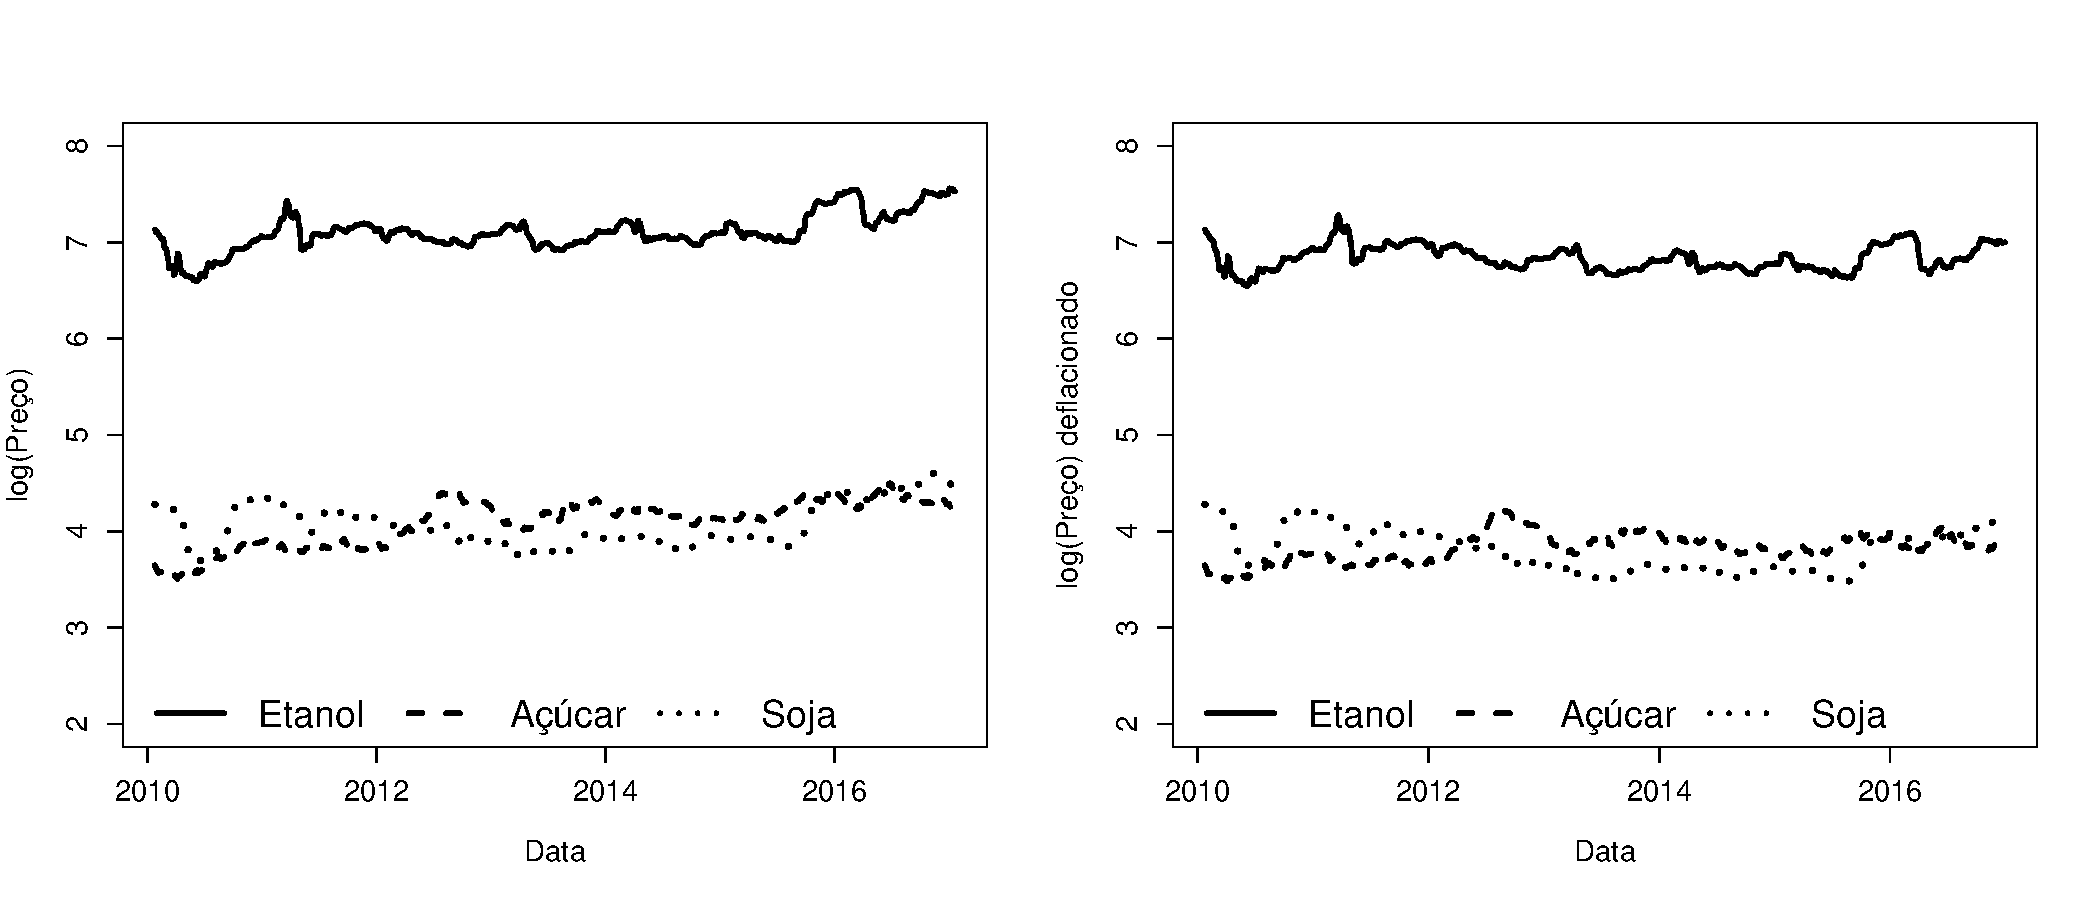
\includegraphics{dados_cepea_files/figure-latex/grafico1-1.pdf}
\caption{Logarítimo dos preços diários e preço diário deflacionado pelo
Ìndice de Preço do Produtor (IPP) para o etanol, açúcar e soja}
\end{figure}

\begin{figure}[htbp]
\centering
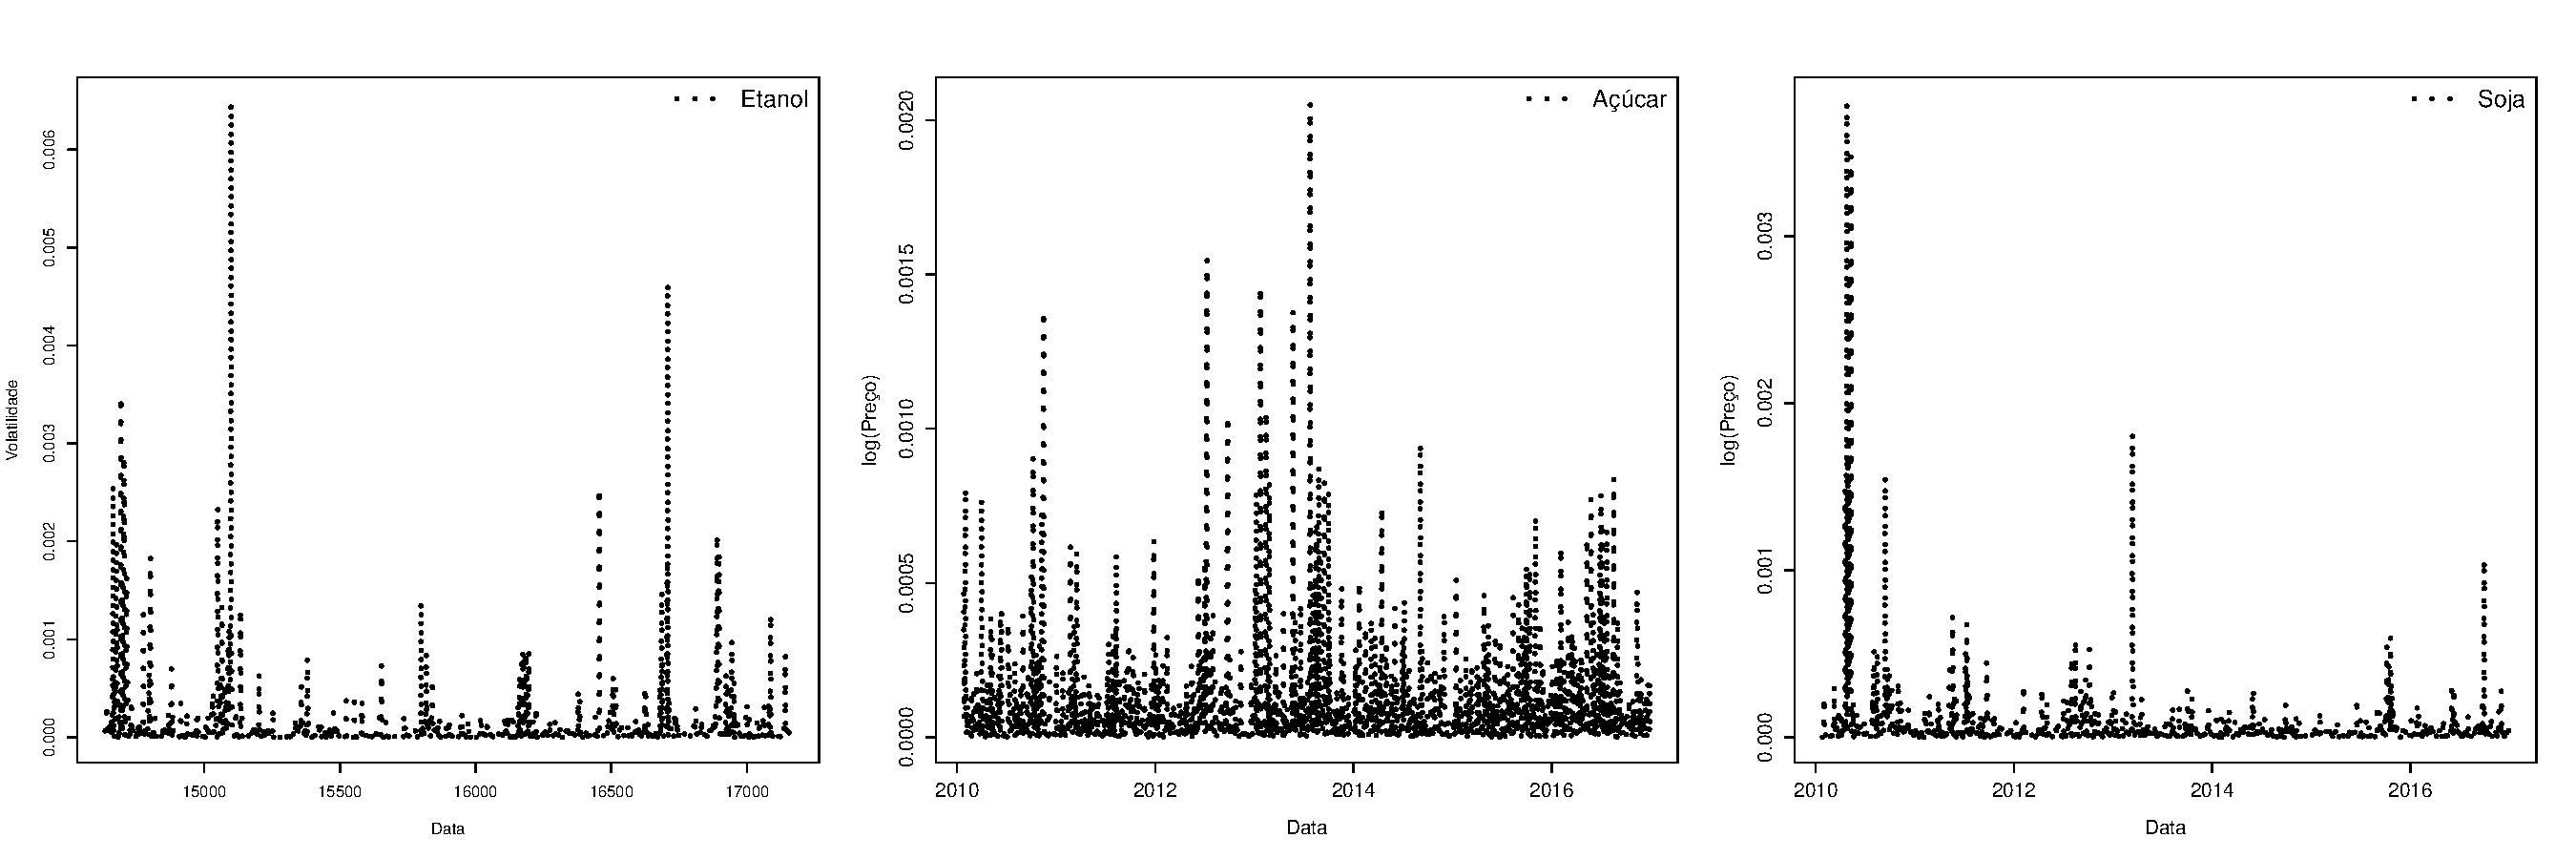
\includegraphics{dados_cepea_files/figure-latex/grafico2-1.pdf}
\caption{Volatilidade medida pela diferença do logarítimo do preço ao
quadrado para a etanol, açúcar e soja}
\end{figure}

\begin{verbatim}
## [1] "Mean"
\end{verbatim}

\begin{verbatim}
##    etanol    acucar      soja 
## 938.48581  46.35046  45.81921
\end{verbatim}

\begin{verbatim}
## [1] "St.D."
\end{verbatim}

\begin{verbatim}
##           etanol   acucar     soja
## etanol 126.37033      NaN 28.34079
## acucar       NaN 6.819198      NaN
## soja    28.34079      NaN 10.63687
\end{verbatim}

\begin{verbatim}
## [1] "Corr."
\end{verbatim}

\begin{verbatim}
##            etanol     acucar       soja
## etanol  1.0000000 -0.2186233  0.5975373
## acucar -0.2186233  1.0000000 -0.4075903
## soja    0.5975373 -0.4075903  1.0000000
\end{verbatim}

\begin{verbatim}
## [1] "Skewness"
\end{verbatim}

\begin{verbatim}
## [1] -0.2896277 -0.1595681 -1.0635649
\end{verbatim}

\begin{verbatim}
## [1] "Kurtosis"
\end{verbatim}

\begin{verbatim}
## [1] 12.333846  4.283914 12.858063
\end{verbatim}

\begin{verbatim}
## [1] "Box Ljung (residuals)"
\end{verbatim}

\begin{verbatim}
## [1] 0.000000e+00 5.107026e-15 0.000000e+00
\end{verbatim}

\begin{verbatim}
## [1] "Box-Ljung (squared residuals)"
\end{verbatim}

\begin{verbatim}
## [1] 0.000000e+00 2.233032e-07 0.000000e+00
\end{verbatim}

\begin{verbatim}
## [1] "ARCH"
\end{verbatim}

\begin{verbatim}
##  Chi-squared  Chi-squared  Chi-squared 
## 0.0000000000 0.0006158753 0.0000000000
\end{verbatim}

\begin{verbatim}
## [1] "Shapiro-Wilk"
\end{verbatim}

\begin{verbatim}
## [1] 3.767565e-36 7.597055e-10 2.443580e-30
\end{verbatim}

\begin{longtable}[t]{lrrrrrrr}
\caption{\label{tab:ADF e KPSS nivel}Teste KPSS preço em nível}\\
\toprule
  & etanol & acucar & soja & 1 Pct & 2.5 Pct & 5 Pct & 10 Pct\\
\midrule
Time Trend: & 1.57 & 3.80 & 5.17 & 0.22 & 0.18 & 0.15 & 0.12\\
No Trend: & 1.88 & 10.65 & 9.45 & 0.74 & 0.57 & 0.46 & 0.35\\
\bottomrule
\end{longtable}

\begin{longtable}[t]{lrrrrrrr}
\caption{\label{tab:ADF e KPSS nivel}Teste ADF preço em nível}\\
\toprule
  & etanol & acucar & soja & 1 Pct & 2.5 Pct & 5 Pct & 10 Pct\\
\midrule
Time Trend: & -3.83 & -1.67 & -2.44 & -3.96 & -3.66 & -3.41 & -3.12\\
Constant: & -3.87 & -1.90 & -2.67 & -3.43 & -3.12 & -2.86 & -2.57\\
Neither: & -0.16 & 0.27 & -0.39 & -2.58 & -2.23 & -1.95 & -1.62\\
\bottomrule
\end{longtable}

\begin{longtable}[t]{lrrr}
\caption{\label{tab:ADF e KPSS nivel}Defasagens do teste ADF}\\
\toprule
  & Trend Model & Drift Model & None\\
\midrule
etanol & 2 & 2 & 2\\
acucar & 1 & 1 & 1\\
soja & 6 & 6 & 5\\
\bottomrule
\end{longtable}

\begin{verbatim}
## 
##  Phillips-Perron Unit Root Test
## 
## data:  dados_cepea_deflacionado[, "etanol"]
## Dickey-Fuller Z(alpha) = -18.985, Truncation lag parameter = 8,
## p-value = 0.08703
## alternative hypothesis: stationary
\end{verbatim}

\begin{verbatim}
## 
##  Phillips-Perron Unit Root Test
## 
## data:  dados_cepea_deflacionado[, "acucar"]
## Dickey-Fuller Z(alpha) = -6.7393, Truncation lag parameter = 8,
## p-value = 0.7338
## alternative hypothesis: stationary
\end{verbatim}

\begin{verbatim}
## 
##  Phillips-Perron Unit Root Test
## 
## data:  dados_cepea_deflacionado[, "soja"]
## Dickey-Fuller Z(alpha) = -3.9061, Truncation lag parameter = 8,
## p-value = 0.8919
## alternative hypothesis: stationary
\end{verbatim}

\begin{longtable}[t]{lrrrrrrr}
\caption{\label{tab:ADF e KPSS logdif}Teste KPSS retorno}\\
\toprule
  & etanol & acucar & soja & 1 Pct & 2.5 Pct & 5 Pct & 10 Pct\\
\midrule
Time Trend: & 0.05 & 0.06 & 0.11 & 0.22 & 0.18 & 0.15 & 0.12\\
No Trend: & 0.15 & 0.14 & 0.72 & 0.74 & 0.57 & 0.46 & 0.35\\
\bottomrule
\end{longtable}

\begin{longtable}[t]{lrrrrrrr}
\caption{\label{tab:ADF e KPSS logdif}Teste ADF retorno}\\
\toprule
  & etanol & acucar & soja & 1 Pct & 2.5 Pct & 5 Pct & 10 Pct\\
\midrule
Time Trend: & -15.51 & -25.43 & -9.18 & -3.96 & -3.66 & -3.41 & -3.12\\
Constant: & -15.49 & -25.42 & -9.11 & -3.43 & -3.12 & -2.86 & -2.57\\
Neither: & -15.50 & -25.42 & -9.11 & -2.58 & -2.23 & -1.95 & -1.62\\
\bottomrule
\end{longtable}

\begin{longtable}[t]{lrrr}
\caption{\label{tab:ADF e KPSS logdif}Defasagens do teste ADF}\\
\toprule
  & Trend Model & Drift Model & None\\
\midrule
etanol & 1 & 1 & 1\\
acucar & 1 & 1 & 1\\
soja & 4 & 4 & 4\\
\bottomrule
\end{longtable}

\begin{verbatim}
## 
##  Phillips-Perron Unit Root Test
## 
## data:  ldif_cepea[-1, "etanol"]
## Dickey-Fuller Z(alpha) = -990.04, Truncation lag parameter = 8,
## p-value = 0.01
## alternative hypothesis: stationary
\end{verbatim}

\begin{verbatim}
## 
##  Phillips-Perron Unit Root Test
## 
## data:  ldif_cepea[-1, "acucar"]
## Dickey-Fuller Z(alpha) = -1473.5, Truncation lag parameter = 8,
## p-value = 0.01
## alternative hypothesis: stationary
\end{verbatim}

\begin{verbatim}
## 
##  Phillips-Perron Unit Root Test
## 
## data:  ldif_cepea[-1, "soja"]
## Dickey-Fuller Z(alpha) = -1685.5, Truncation lag parameter = 8,
## p-value = 0.01
## alternative hypothesis: stationary
\end{verbatim}

\begin{verbatim}
## selected order: aic =  7 
## selected order: bic =  4 
## selected order: hq =  6 
## Summary table:  
##        p      AIC      BIC       HQ       M(p) p-value
##  [1,]  0 -11.5960 -11.5960 -11.5960     0.0000  0.0000
##  [2,]  1 -28.4651 -28.4365 -28.4545 28720.4234  0.0000
##  [3,]  2 -28.9585 -28.9014 -28.9374   855.9078  0.0000
##  [4,]  3 -29.0894 -29.0038 -29.0577   239.7097  0.0000
##  [5,]  4 -29.1391 -29.0250 -29.0969   101.8209  0.0000
##  [6,]  5 -29.1570 -29.0143 -29.1042    47.8572  0.0000
##  [7,]  6 -29.1725 -29.0013 -29.1091    43.8599  0.0000
##  [8,]  7 -29.1804 -28.9807 -29.1065    31.0196  0.0003
##  [9,]  8 -29.1738 -28.9456 -29.0894     6.4510  0.6941
## [10,]  9 -29.1677 -28.9109 -29.0727     7.2904  0.6069
## [11,] 10 -29.1624 -28.8771 -29.0568     8.6824  0.4671
## [12,] 11 -29.1553 -28.8415 -29.0392     5.6868  0.7708
## [13,] 12 -29.1497 -28.8073 -29.0230     8.0703  0.5271
## [14,] 13 -29.1438 -28.7729 -29.0066     7.6895  0.5657
\end{verbatim}

\begin{verbatim}
## 
## ###################### 
## # Johansen-Procedure # 
## ###################### 
## 
## Test type: trace statistic , with linear trend 
## 
## Eigenvalues (lambda):
## [1] 0.016725504 0.005288100 0.002397643
## 
## Values of teststatistic and critical values of test:
## 
##           test 10pct  5pct  1pct
## r <= 2 |  4.12  6.50  8.18 11.65
## r <= 1 | 13.22 15.66 17.95 23.52
## r = 0  | 42.16 28.71 31.52 37.22
## 
## Eigenvectors, normalised to first column:
## (These are the cointegration relations)
## 
##             etanol.l3  acucar.l3    soja.l3
## etanol.l3  1.00000000   1.000000  1.0000000
## acucar.l3 -0.02988903 -19.561243 -0.8718529
## soja.l3   -0.31575726  -3.996291 -4.4371453
## 
## Weights W:
## (This is the loading matrix)
## 
##             etanol.l3     acucar.l3      soja.l3
## etanol.d -0.009108278 -1.126194e-04 2.354312e-05
## acucar.d -0.005376216  1.926758e-04 2.252981e-04
## soja.d    0.001030792 -5.708165e-05 3.441345e-04
\end{verbatim}

\begin{verbatim}
## 
## ##################################################### 
## # Johansen-Procedure Unit Root / Cointegration Test # 
## ##################################################### 
## 
## The value of the test statistic is: 4.1193 13.2178 42.1614
\end{verbatim}

\begin{verbatim}
## [1] "VECM ols"
\end{verbatim}

\begin{verbatim}
## alpha:  
##        etanol   acucar    soja
## [1,] -0.00968 -0.00529 0.00104
## standard error 
##         [,1]    [,2]    [,3]
## [1,] 0.00195 0.00215 0.00151
## AR coefficient matrix 
## AR( 1 )-matrix 
##         etanol  acucar     soja
## etanol  0.3730 -0.0543 -0.00696
## acucar -0.0145  0.1943  0.02106
## soja    0.0171  0.0154  0.21612
## standard error 
##        [,1]   [,2]   [,3]
## [1,] 0.0241 0.0221 0.0307
## [2,] 0.0265 0.0243 0.0338
## [3,] 0.0186 0.0171 0.0237
## AR( 2 )-matrix 
##        etanol  acucar    soja
## etanol 0.2617 -0.0101 -0.0283
## acucar 0.0165  0.0184  0.0104
## soja   0.0602 -0.0274  0.1748
## standard error 
##        [,1]   [,2]   [,3]
## [1,] 0.0250 0.0225 0.0309
## [2,] 0.0275 0.0248 0.0340
## [3,] 0.0193 0.0174 0.0239
## AR( 3 )-matrix 
##          etanol    acucar    soja
## etanol  0.03512 -0.042739  0.0296
## acucar -0.00229  0.010066 -0.0165
## soja   -0.01668 -0.000225  0.2327
## standard error 
##        [,1]   [,2]   [,3]
## [1,] 0.0243 0.0221 0.0306
## [2,] 0.0268 0.0244 0.0337
## [3,] 0.0188 0.0171 0.0237
## ----- 
## Residuals cov-mtx: 
##              etanol       acucar         soja
## etanol 6.714620e-05 3.961111e-06 4.825925e-06
## acucar 3.961111e-06 8.148757e-05 7.242273e-06
## soja   4.825925e-06 7.242273e-06 4.014542e-05
##        
## det(sse) =  2.138862e-13 
## AIC =  -29.13843 
## BIC =  -29.04332
\end{verbatim}

\begin{verbatim}
## [1] "Refinamento VECM ols"
\end{verbatim}

\begin{verbatim}
## Equation:  1  npar =  6 
## Equation:  2  npar =  2 
## Equation:  3  npar =  5 
## alpha:  
##          [,1]     [,2] [,3]
## [1,] -0.00964 -0.00537    0
## standard error 
##         [,1]    [,2] [,3]
## [1,] 0.00195 0.00212    1
## AR coefficient matrix 
## AR( 1 )-matrix 
##       [,1]    [,2] [,3]
## [1,] 0.373 -0.0574 0.00
## [2,] 0.000  0.2000 0.00
## [3,] 0.000  0.0000 0.22
## standard error 
##        [,1]   [,2]   [,3]
## [1,] 0.0239 0.0215 1.0000
## [2,] 1.0000 0.0237 1.0000
## [3,] 1.0000 1.0000 0.0234
## AR( 2 )-matrix 
##        [,1]    [,2]  [,3]
## [1,] 0.2584  0.0000 0.000
## [2,] 0.0000  0.0000 0.000
## [3,] 0.0613 -0.0259 0.174
## standard error 
##        [,1]   [,2]   [,3]
## [1,] 0.0248 1.0000 1.0000
## [2,] 1.0000 1.0000 1.0000
## [3,] 0.0154 0.0167 0.0239
## AR( 3 )-matrix 
##        [,1]    [,2] [,3]
## [1,] 0.0368 -0.0432 0.00
## [2,] 0.0000  0.0000 0.00
## [3,] 0.0000  0.0000 0.23
## standard error 
##        [,1]   [,2]   [,3]
## [1,] 0.0241 0.0216 1.0000
## [2,] 1.0000 1.0000 1.0000
## [3,] 1.0000 1.0000 0.0234
## ----- 
## Residuals cov-mtx: 
##              [,1]         [,2]         [,3]
## [1,] 6.721523e-05 3.909699e-06 4.830615e-06
## [2,] 3.909699e-06 8.158966e-05 7.222317e-06
## [3,] 4.830615e-06 7.222317e-06 4.020320e-05
##        
## det(sse) =  2.147254e-13 
## AIC =  -29.15429 
## BIC =  -29.11308
\end{verbatim}

\begin{verbatim}
## [1] "VECM MLL"
\end{verbatim}

\begin{verbatim}
## Order p:  4  Co-integrating rank:  1 
## Number of parameters:  32 
## initial estimates:  -0.009374727 -0.003209131 0.0004045168 -0.3 -0.316 0.3715428 -0.05441418 -0.009196336 0.2603996 -0.01078983 -0.03067087 0.03377289 -0.04367577 0.02684032 -0.01415261 0.1955592 0.01988912 0.01516204 0.01949997 0.009045315 -0.005428375 0.01142869 -0.0176619 0.01692267 0.01499143 0.2163395 0.06051098 -0.02782985 0.1751025 -0.01577921 -0.0007107781 0.2328644 
## Par. Lower-bounds:  -0.01210885 -0.006225814 -0.001710967 -0.3361787 -0.3521787 0.3354285 -0.08751872 -0.05521036 0.2229197 -0.04453053 -0.07692977 -0.002596274 -0.07687652 -0.01902405 -0.05399908 0.1590335 -0.03088018 -0.02619119 -0.01772764 -0.04199418 -0.04555608 -0.02520318 -0.06826609 -0.01102011 -0.01062264 0.180737 0.03151155 -0.05393613 0.1393105 -0.04391922 -0.02639929 0.1973776 
## Par. Upper-bounds:  -0.0066406 -0.0001924473 0.00252 -0.2638213 -0.2798213 0.407657 -0.02130963 0.03681769 0.2978795 0.02295087 0.01558804 0.07014205 -0.01047501 0.0727047 0.02569385 0.2320849 0.07065842 0.05651527 0.05672757 0.06008481 0.03469933 0.04806055 0.0329423 0.04486546 0.0406055 0.2519421 0.0895104 -0.001723563 0.2108946 0.0123608 0.02497774 0.2683512 
## Final   Estimates:  -0.0066406 -0.0004365751 -0.0004796343 -0.3361787 -0.3521787 0.3704735 -0.02950388 -0.05521036 0.2358613 0.01218878 -0.05401157 0.02960165 -0.02220414 -0.01902405 -0.01451443 0.2030534 0.005419323 0.007583905 0.02144373 -0.001978513 -0.01481176 0.01382601 -0.03041673 0.01073457 0.01574557 0.2160566 0.05069935 -0.03154683 0.1685565 -0.007705943 -0.001910744 0.2271728 
## 
## Coefficient(s):
##         Estimate  Std. Error  t value Pr(>|t|)    
##  [1,] -0.0066406          NA       NA       NA    
##  [2,] -0.0004366   0.0001828   -2.388 0.016946 *  
##  [3,] -0.0004796   0.0001273   -3.768 0.000165 ***
##  [4,] -0.3361787   0.3382068   -0.994 0.320221    
##  [5,] -0.3521787   0.3412452   -1.032 0.302053    
##  [6,]  0.3704735   0.0855833    4.329 1.50e-05 ***
##  [7,] -0.0295039   0.0783249   -0.377 0.706407    
##  [8,] -0.0552104   0.1090822   -0.506 0.612762    
##  [9,]  0.2358613   0.0888778    2.654 0.007960 ** 
## [10,]  0.0121888   0.0797436    0.153 0.878517    
## [11,] -0.0540116   0.1095726   -0.493 0.622062    
## [12,]  0.0296017   0.0858413    0.345 0.730213    
## [13,] -0.0222041   0.0784180   -0.283 0.777061    
## [14,] -0.0190241   0.1086289   -0.175 0.860978    
## [15,] -0.0145144   0.0271424   -0.535 0.592821    
## [16,]  0.2030534   0.0248698    8.165 2.22e-16 ***
## [17,]  0.0054193   0.0345212    0.157 0.875256    
## [18,]  0.0075839   0.0281935    0.269 0.787934    
## [19,]  0.0214437   0.0253255    0.847 0.397149    
## [20,] -0.0019785   0.0341446   -0.058 0.953792    
## [21,] -0.0148118   0.0272380   -0.544 0.586586    
## [22,]  0.0138260   0.0248891    0.556 0.578549    
## [23,] -0.0304167   0.0344829   -0.882 0.377733    
## [24,]  0.0107346   0.0194915    0.551 0.581819    
## [25,]  0.0157456   0.0178546    0.882 0.377844    
## [26,]  0.2160566   0.0248678    8.688  < 2e-16 ***
## [27,]  0.0506994   0.0202497    2.504 0.012290 *  
## [28,] -0.0315468   0.0181912   -1.734 0.082885 .  
## [29,]  0.1685565   0.0249822    6.747 1.51e-11 ***
## [30,] -0.0077059   0.0195501   -0.394 0.693461    
## [31,] -0.0019107   0.0178543   -0.107 0.914774    
## [32,]  0.2271728   0.0247883    9.165  < 2e-16 ***
## ---
## Signif. codes:  0 '***' 0.001 '**' 0.01 '*' 0.05 '.' 0.1 ' ' 1
## alpha:  
##           [,1]
## [1,] -0.006641
## [2,] -0.000437
## [3,] -0.000480
## standard error 
##          [,1]
## [1,]      NaN
## [2,] 0.000183
## [3,] 0.000127
## beta:  
##        [,1]
## [1,]  1.000
## [2,] -0.336
## [3,] -0.352
## standard error 
##       [,1]
## [1,] 1.000
## [2,] 0.338
## [3,] 0.341
## AR coefficient matrix 
## AR( 1 )-matrix 
##         [,1]    [,2]     [,3]
## [1,]  0.3705 -0.0295 -0.05521
## [2,] -0.0145  0.2031  0.00542
## [3,]  0.0107  0.0157  0.21606
## standard error 
##        [,1]   [,2]   [,3]
## [1,] 0.0856 0.0783 0.1091
## [2,] 0.0271 0.0249 0.0345
## [3,] 0.0195 0.0179 0.0249
## AR( 2 )-matrix 
##         [,1]    [,2]     [,3]
## [1,] 0.23586  0.0122 -0.05401
## [2,] 0.00758  0.0214 -0.00198
## [3,] 0.05070 -0.0315  0.16856
## standard error 
##        [,1]   [,2]   [,3]
## [1,] 0.0889 0.0797 0.1096
## [2,] 0.0282 0.0253 0.0341
## [3,] 0.0202 0.0182 0.0250
## AR( 3 )-matrix 
##          [,1]     [,2]    [,3]
## [1,]  0.02960 -0.02220 -0.0190
## [2,] -0.01481  0.01383 -0.0304
## [3,] -0.00771 -0.00191  0.2272
## standard error 
##        [,1]   [,2]   [,3]
## [1,] 0.0858 0.0784 0.1086
## [2,] 0.0272 0.0249 0.0345
## [3,] 0.0196 0.0179 0.0248
## ----- 
## Residuals cov-mtx: 
##              etanol       acucar         soja
## etanol 8.464302e-04 5.735088e-05 5.955313e-05
## acucar 5.735088e-05 8.526871e-05 1.091269e-05
## soja   5.955313e-05 1.091269e-05 4.396170e-05
##        
## det(sse) =  2.699629e-12 
## AIC =  -26.60068 
## BIC =  -26.49923
\end{verbatim}

\begin{verbatim}
## [1] "Refinamento VECM MLL"
\end{verbatim}

\begin{verbatim}
## Order p:  4  Co-integrating rank:  1 
## Number of parameters:  13 
## initial estimates:  -0.0066406 -0.0004365751 -0.0004796343 -0.3361787 -0.3521787 0.3704735 0.2358613 0.2030534 0.2160566 0.05069935 -0.03154683 0.1685565 0.2271728 
## Par. Lower-bounds:  NaN -0.0007108197 -0.0006705721 -0.3723575 -0.3883575 0.2420985 0.1025446 0.1657487 0.1787549 0.02032478 -0.05883356 0.1310832 0.1899903 
## Par. Upper-bounds:  NaN -0.0001623304 -0.0002886965 -0.3 -0.316 0.4988485 0.369178 0.240358 0.2533582 0.08107393 -0.004260103 0.2060298 0.2643553 
## Final   Estimates:  -0.0066406 -0.0001623304 -0.0002886965 -0.3723575 -0.3883575 0.2420985 0.369178 0.240358 0.2533582 0.08107393 -0.004260103 0.2060298 0.2643553 
## 
## Coefficient(s):
##         Estimate  Std. Error  t value Pr(>|t|)    
##  [1,] -0.0066406          NA       NA       NA    
##  [2,] -0.0001623   0.0001826   -0.889  0.37413    
##  [3,] -0.0002887   0.0001290   -2.238  0.02524 *  
##  [4,] -0.3723575   0.3174371   -1.173  0.24079    
##  [5,] -0.3883575   0.3202451   -1.213  0.22525    
##  [6,]  0.2420985   0.0751525    3.221  0.00128 ** 
##  [7,]  0.3691780   0.0768190    4.806 1.54e-06 ***
##  [8,]  0.2403580   0.0235197   10.219  < 2e-16 ***
##  [9,]  0.2533582   0.0233280   10.861  < 2e-16 ***
## [10,]  0.0810739   0.0156425    5.183 2.18e-07 ***
## [11,] -0.0042601   0.0165967   -0.257  0.79742    
## [12,]  0.2060298   0.0237682    8.668  < 2e-16 ***
## [13,]  0.2643553   0.0233053   11.343  < 2e-16 ***
## ---
## Signif. codes:  0 '***' 0.001 '**' 0.01 '*' 0.05 '.' 0.1 ' ' 1
## alpha:  
##           [,1]
## [1,] -0.006641
## [2,] -0.000162
## [3,] -0.000289
## standard error 
##          [,1]
## [1,]      NaN
## [2,] 0.000183
## [3,] 0.000129
## beta:  
##        [,1]
## [1,]  1.000
## [2,] -0.372
## [3,] -0.388
## standard error 
##       [,1]
## [1,] 1.000
## [2,] 0.317
## [3,] 0.320
## AR coefficient matrix 
## AR( 1 )-matrix 
##       [,1] [,2]  [,3]
## [1,] 0.242 0.00 0.000
## [2,] 0.000 0.24 0.000
## [3,] 0.000 0.00 0.253
## standard error 
##        [,1]   [,2]   [,3]
## [1,] 0.0752 1.0000 1.0000
## [2,] 1.0000 0.0235 1.0000
## [3,] 1.0000 1.0000 0.0233
## AR( 2 )-matrix 
##        [,1]     [,2]  [,3]
## [1,] 0.3692  0.00000 0.000
## [2,] 0.0000  0.00000 0.000
## [3,] 0.0811 -0.00426 0.206
## standard error 
##        [,1]   [,2]   [,3]
## [1,] 0.0768 1.0000 1.0000
## [2,] 1.0000 1.0000 1.0000
## [3,] 0.0156 0.0166 0.0238
## AR( 3 )-matrix 
##      [,1] [,2]  [,3]
## [1,]    0    0 0.000
## [2,]    0    0 0.000
## [3,]    0    0 0.264
## standard error 
##      [,1] [,2]   [,3]
## [1,]    1    1 1.0000
## [2,]    1    1 1.0000
## [3,]    1    1 0.0233
## ----- 
## Residuals cov-mtx: 
##              etanol       acucar         soja
## etanol 7.498651e-04 2.248021e-05 3.363317e-05
## acucar 2.248021e-05 8.234223e-05 7.809303e-06
## soja   3.363317e-05 7.809303e-06 4.177998e-05
##        
## det(sse) =  2.431548e-12 
## AIC =  -26.72737 
## BIC =  -26.68616
\end{verbatim}

\pagebreak

\section*{Referências}\label{referencias}
\addcontentsline{toc}{section}{Referências}

\setlength{\parindent}{0in}

\hypertarget{refs}{}
\hypertarget{ref-lopez_cabrera_volatility_2016}{}
López Cabrera, Brenda, and Franziska Schulz. 2016. ``Volatility Linkages
Between Energy and Agricultural Commodity Prices.'' \emph{Energy
Economics} 54 (February): 190--203.
doi:\href{https://doi.org/10.1016/j.eneco.2015.11.018}{10.1016/j.eneco.2015.11.018}.

\hypertarget{ref-zeileis_zoo:_2005}{}
Zeileis, Achim, and Gabor Grothendieck. 2005. ``Zoo: S3 Infrastructure
for Regular and Irregular Time Series.'' \emph{Journal of Statistical
Software} 014 (i06): 1--27.
doi:\href{https://doi.org/10.18637/jss.v014.i06}{10.18637/jss.v014.i06}.


\end{document}
